\chapter{Aging, Hysteresis, and Voltage Protocols}

\section{Aging and Measurement Timescales}

The model separates slow degradation from fast J--V measurement. The aging
voltage $V_{\mathrm{stress}}(t)$ defines the electrical bias under which the
device is held during degradation. The measurement voltage
$V_{\mathrm{app}}(t)$ defines the time-dependent sweep used to extract a J--V
curve. These two voltages are not interchangeable. A device may age under one
bias condition and then be measured under a separate scan protocol at selected
ages.

The fast timescale is the J--V scan timescale, over which the applied voltage
changes and mobile ions may redistribute. The slow timescale is the aging
timescale, over which damage states such as trap growth, contact degradation,
and shunt formation evolve. The COMSOL study sequence therefore alternates
between stress periods and measurement periods:
\begin{enumerate}
\item hold the device at a stress condition such as light plus heat and
$V_{\mathrm{stress}}$;
\item apply a reset or pre-bias condition to define the initial scan state;
\item run a forward, reverse, or bidirectional J--V scan using
$V_{\mathrm{app}}(t)$;
\item return the model to the aging voltage; and
\item repeat the measurement at selected degradation states.
\end{enumerate}

\section{Accelerated Aging Interpretation}

The accelerated 60 s COMSOL simulation is not equivalent to real 60 s aging.
It is a compressed demonstration in which degradation rates are scaled so that
the direction and shape of degradation can be studied within a practical
simulation time. The acceleration factor is
\begin{equation}
\mathrm{DegAccel}=\frac{t_{\mathrm{real}}}{t_{\mathrm{sim}}}.
\end{equation}
The physical interpretation of each component is:
\begin{itemize}
\item $\xion$: reversible ionic-screening state that captures field
redistribution, hysteresis, and quasi-static interfacial charge
accumulation,
\item $\xbulk$: irreversible bulk-damage state that captures trap growth,
carrier lifetime loss, and optional photogeneration loss,
\item $\xint$: irreversible interface/contact-damage state that captures
contact degradation, leakage growth, interfacial recombination growth, and
electrode-driven failure pathways.
\end{itemize}

\subsection{Conserved Mobile-Ion Inventory Assumption}

The ionic state $\xion$ is not interpreted as a change in the total mobile-ion
concentration over the lifetime of the simulated device. Instead, it is a
low-order measure of how strongly a conserved population of mobile ions has
redistributed and screened the internal electric field. This distinction is
important because standard drift--diffusion PSC ion-migration models describe
mobile ionic vacancies using a continuity equation with blocking, no-flux
boundary conditions at the perovskite interfaces \cite{Courtier_2017}:
\begin{equation}
\frac{\partial c_{\mathrm{ion}}}{\partial t}
+ \frac{\partial \mathcal{F}_{\mathrm{ion}}}{\partial x}=0,
\qquad
\mathcal{F}_{\mathrm{ion}}(0,t)=
\mathcal{F}_{\mathrm{ion}}(L_{\mathrm{pvk}},t)=0.
\end{equation}
Integrating across the absorber gives
\begin{equation}
\frac{d}{dt}\int_{0}^{L_{\mathrm{pvk}}}
 c_{\mathrm{ion}}(x,t)\,dx
= -\mathcal{F}_{\mathrm{ion}}(L_{\mathrm{pvk}},t)
+ \mathcal{F}_{\mathrm{ion}}(0,t)=0.
\end{equation}
Therefore, the total mobile-ion inventory remains constant in the ion-motion
submodel, while the spatial ion profile, interfacial charge accumulation, and
field screening can change with bias, illumination, and temperature. In this
thesis, degradation is therefore allowed to change the effectiveness and
consequences of ionic redistribution, but it does not create or destroy mobile
ions unless an explicit source, sink, chemical generation, annihilation, or
volatile-loss term is added to the model.

For reporting convenience, a scalar observable
\begin{equation}
\Dmaster = w_{\mathrm{ion}}\xion + w_{\mathrm{bulk}}\xbulk + w_{\mathrm{int}}\xint
\end{equation}
may still be defined, but it is no longer the primary dynamical object.
Instead, it serves only as a compact summary metric when a single index is
needed for plots or optimization outputs.

For example,
\begin{equation}
24~\mathrm{h}=86400~\mathrm{s},
\end{equation}
so compressing 24 h into 60 s gives
\begin{equation}
\mathrm{DegAccel}=\frac{86400}{60}=1440.
\end{equation}
If a 1000 h $T_{80}$ trajectory is compressed into 60 s, then
\begin{equation}
\mathrm{DegAccel}
=\frac{1000\cdot 3600}{60}
=60000.
\end{equation}
These factors define computational acceleration, not physical time equivalence.
Any lifetime claim requires calibration of degradation rates against matched
experimental aging data.

\section{Degradation Scenario Library}

The degradation library uses a master degradation coordinate as a compact
simulation control:
\begin{equation}
\Dmaster(t)=1-\exp\left(-t/\tau_{\mathrm{deg}}\right).
\end{equation}
This coordinate is dimensionless and bounded between 0 and 1. It is mapped into
controlled changes in $R_s$, $R_{sh}$, $N_t$, fixed or ionic charge, surface
recombination, and photogeneration. The coordinate itself is not interpreted as
a unique physical damage mechanism. It is a numerical driver used to activate
mechanism-specific parameter mappings.

The scenario matrix supports all-off, full coupled, one-mechanism, and
leave-one-out studies. The all-off control tests whether the processing path
creates artificial degradation. One-mechanism cases isolate the J--V signature
of a single parameter mapping. Leave-one-out cases test whether the coupled
response is additive, counteracting, or dominated by interactions.

\section{Scan-Rate-Dependent J--V Protocol}

Scan-rate-dependent J--V behavior requires a time-dependent voltage program
rather than a static voltage sweep. In a static sweep, the internal ionic state
is effectively fixed or assumed equilibrated at each voltage point. In a
time-dependent scan, mobile ions evolve while the voltage changes, so the
measured curve depends on scan direction and scan rate.

The hysteresis protocol contains four segments:
\begin{enumerate}
\item pre-bias hold to establish an initial ionic and electrostatic state;
\item reverse scan from high voltage toward low voltage;
\item low-voltage hold or rest period; and
\item forward scan back toward high voltage.
\end{enumerate}

\begin{figure}[H]
\centering
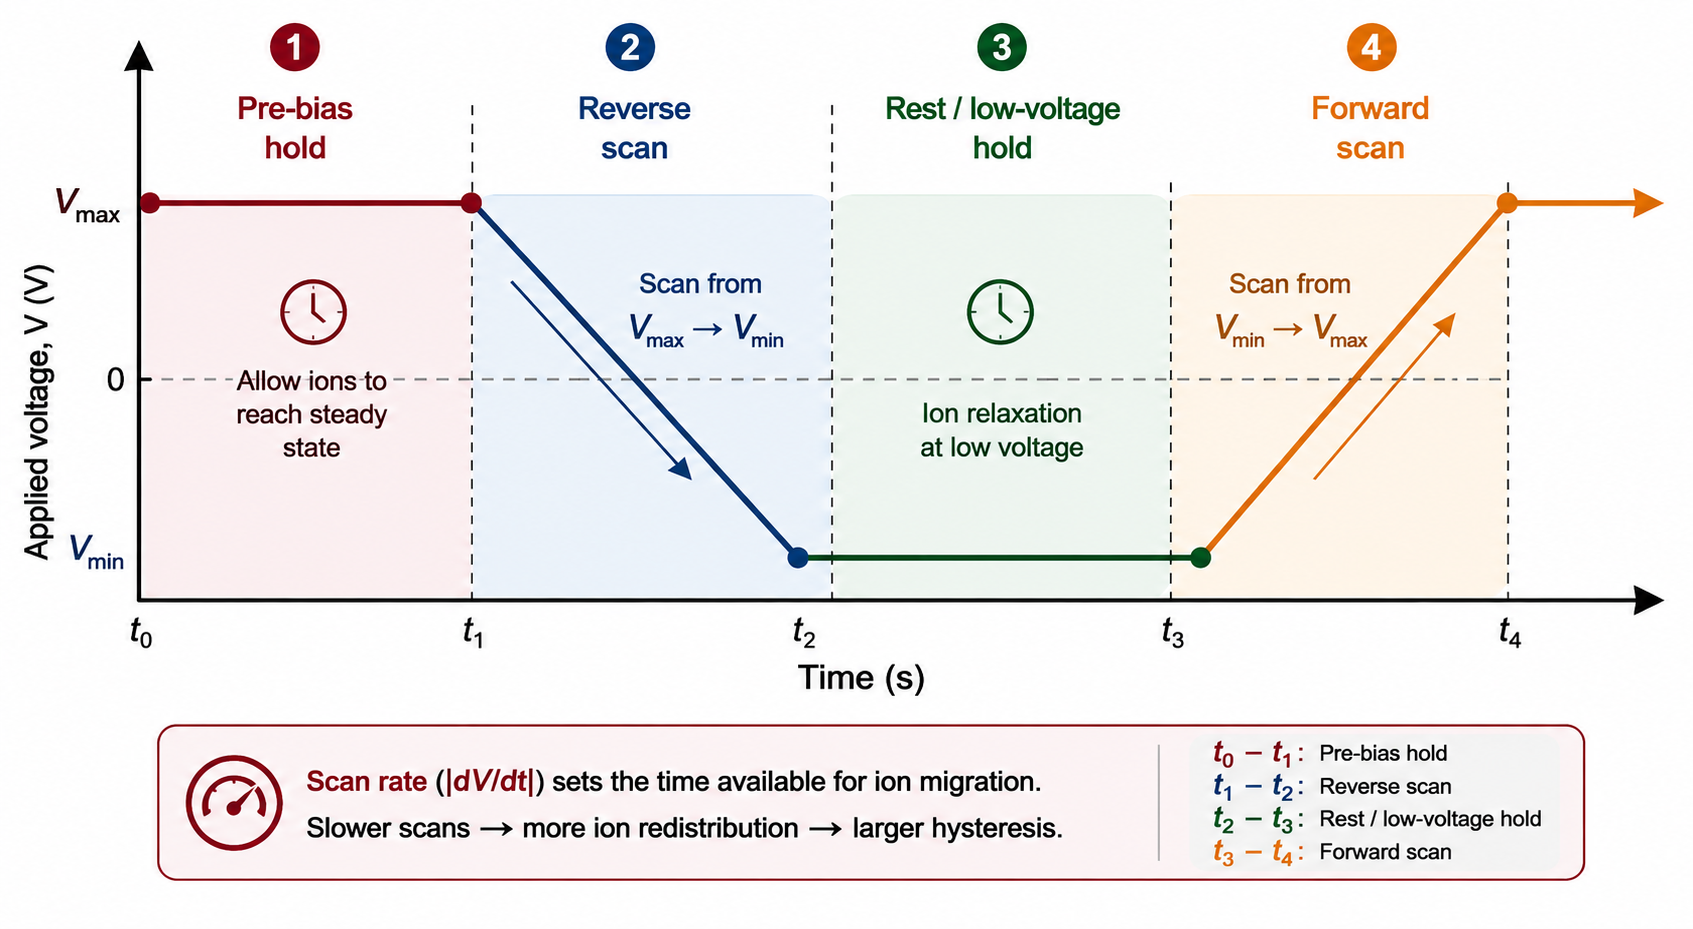
\includegraphics[width=\textwidth]{figures/pptx_ai/jv_scan_protocol_graphic.png}
\caption{Time-dependent J--V scan protocol used for hysteresis simulation. The pre-bias hold defines the initial ionic state, the reverse scan and forward scan impose finite scan-rate dynamics, and the low-voltage hold allows partial ion relaxation before the return sweep.}
\label{fig:voltage_programs}
\end{figure}

The presentation case uses a mobile-ion concentration
\begin{equation}
N_0 = 10^{17}~\mathrm{cm^{-3}},
\end{equation}
ion mobility
\begin{equation}
\mu_{\mathrm{ion}} = 10^{-18}~\mathrm{m^2/(V\,s)},
\end{equation}
and scan rate
\begin{equation}
r_{\mathrm{scan}}=0.1~\mathrm{V/s}.
\end{equation}
Slower scans allow more ion redistribution during the measurement, which can
increase the separation between forward and reverse scans. The simulated
hysteresis result shows that mobile-ion redistribution modifies the internal
field during measurement. It does not yet prove that the chosen ion mobility,
ion concentration, or ion--trap coupling is experimentally unique.

\begin{figure}[H]
\centering
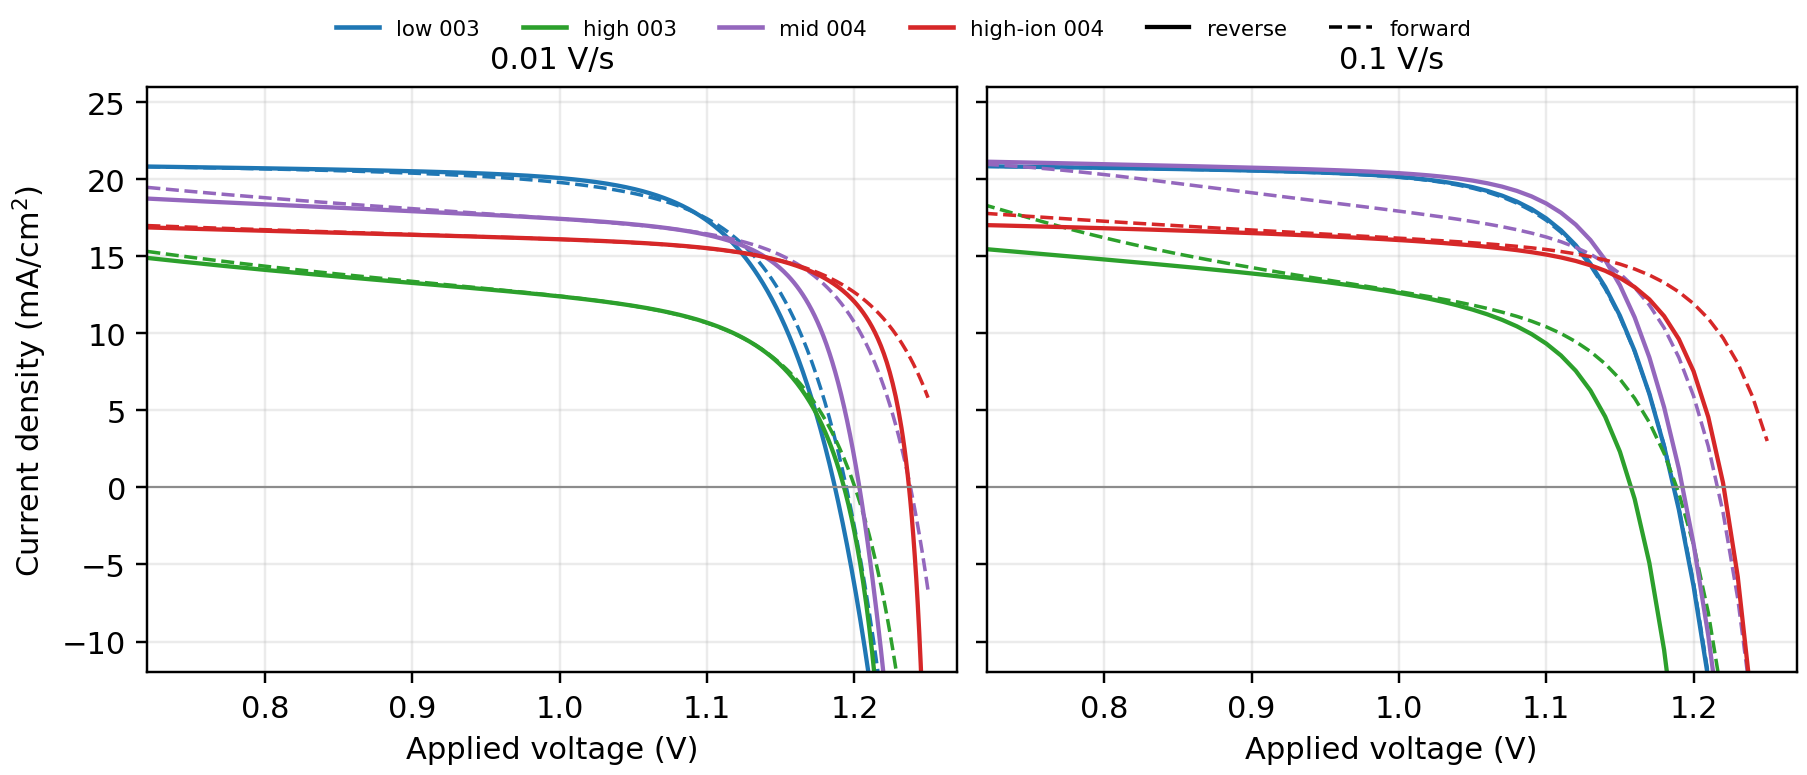
\includegraphics[width=0.78\textwidth]{figures/eee598_comsol/jv_curves.png}
\caption{Representative forward and reverse J--V scans from the multi-rate COMSOL hysteresis study. The scan-direction dependence indicates that the internal electrostatic state changes during the measurement.}
\label{fig:hysteretic_jv}
\end{figure}

\section{DIT Pulse and Mobile-Ion Concentration Extraction}

The drift-ion transient (DIT) protocol provides an ion-sensitive complement to
multi-rate J--V scans. A preconditioned ionic profile is perturbed with a short
voltage pulse, the terminal current transient is recorded, and the mobile-ion
charge associated with the transient component is integrated
\cite{Futscher_2019,SchmidtPRX_2025,SchmidtACS_2025}. In COMSOL, the protocol
is implemented as a time-dependent voltage boundary condition:
\begin{equation}
V_{\mathrm{DIT}}(t)=
\begin{cases}
V_{\mathrm{base}}, & t<t_{\mathrm{on}},\\
V_{oc}, & t_{\mathrm{on}}\le t<t_{\mathrm{off}},\\
V_{\mathrm{base}}, & t\ge t_{\mathrm{off}},
\end{cases}
\qquad
t_{\mathrm{off}}=t_{\mathrm{on}}+10~\mathrm{ms}.
\label{eq:dit_pulse}
\end{equation}
The pulse function belongs only in the time-dependent study. Stationary
initialization and preconditioning studies use constant voltages because the
stationary solver has no time variable and cannot evaluate a function that
depends on \texttt{t}. The DIT study is initialized from the preconditioned
$u_{\mathrm{ion}}(x,0)$ profile and then applies $V_{\mathrm{DIT}}(t)$ to the
terminal or external-circuit boundary.

\begin{figure}[H]
\centering
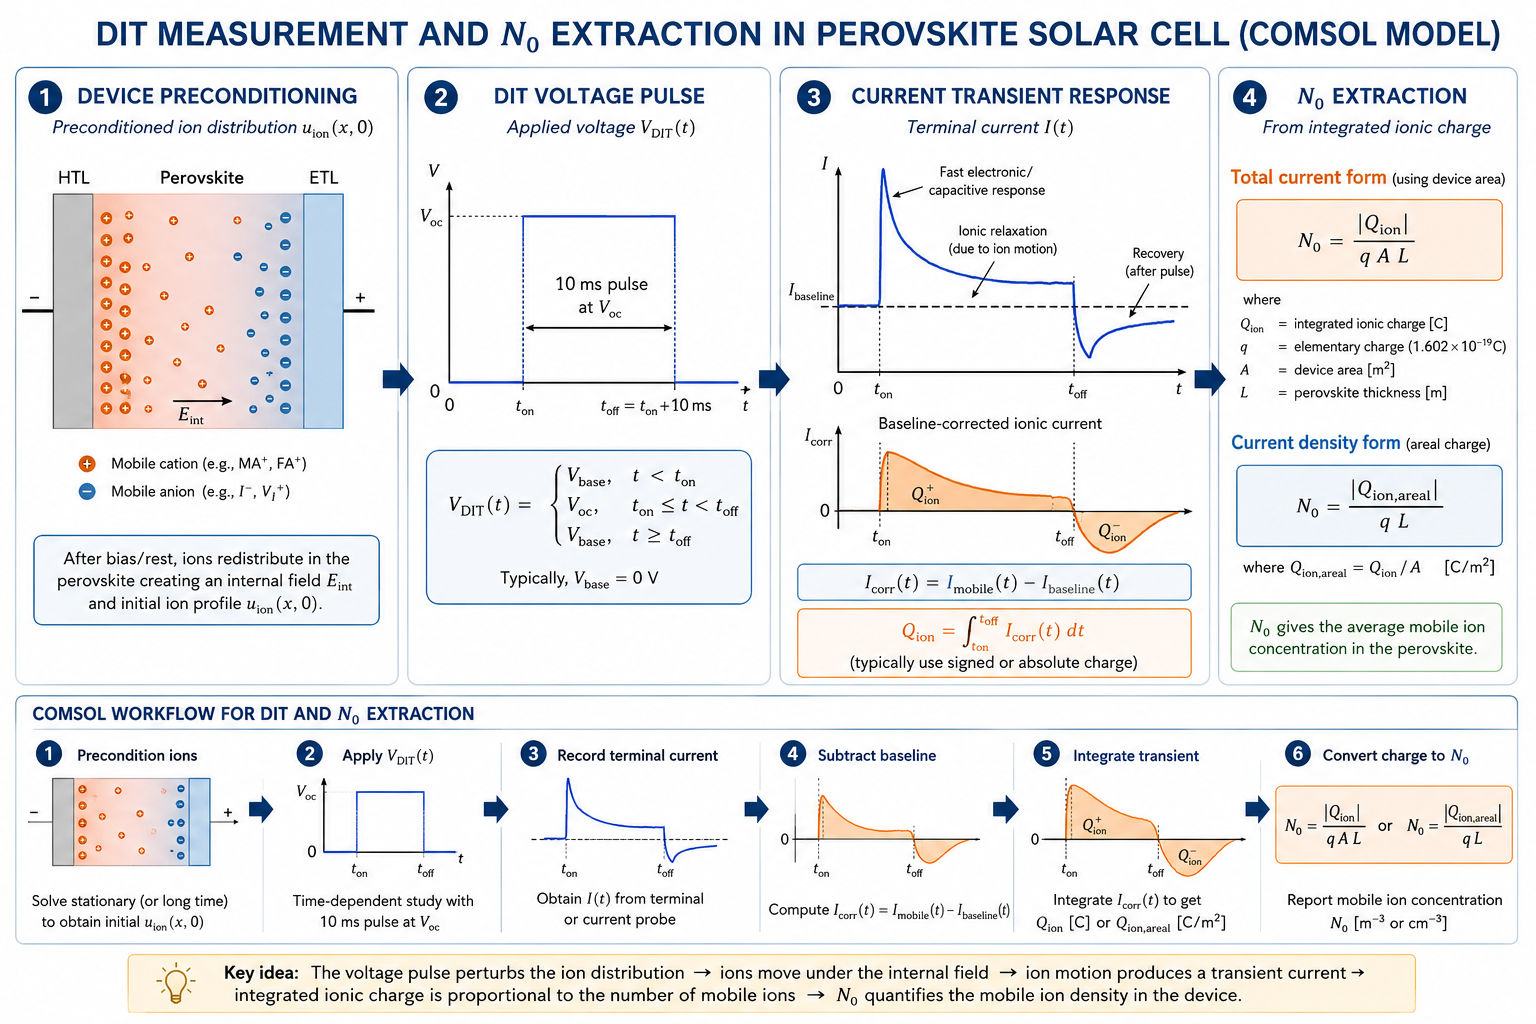
\includegraphics[width=\textwidth]{figures/dit_n0_extraction_infographic.png}
\caption{DIT measurement concept and COMSOL extraction workflow. A preconditioned ion profile is perturbed by a 10 ms voltage pulse, the baseline-corrected current transient is integrated, and the integrated ionic charge is converted into an average mobile-ion concentration.}
\label{fig:dit_n0_extraction}
\end{figure}

The recorded terminal current contains fast electronic, capacitive, leakage,
and ionic contributions. The ion-sensitive quantity is therefore not the raw
current plateau but a baseline-corrected transient:
\begin{equation}
I_{\mathrm{corr}}(t)
=I_{\mathrm{mobile}}(t)-I_{\mathrm{baseline}}(t).
\end{equation}
The best baseline is obtained from an otherwise identical frozen-ion or
ion-blocked control. If only the mobile-ion simulation is available, subtracting
a steady pulse plateau gives an apparent transient charge rather than a unique
mobile-ion density. For total current, the integrated ionic charge and average
mobile-ion concentration are
\begin{align}
Q_{\mathrm{ion}} &=\int_{t_{\mathrm{on}}}^{t_{\mathrm{off}}}
I_{\mathrm{corr}}(t)\,dt,\\
N_0 &=\frac{|Q_{\mathrm{ion}}|}{qAL},
\end{align}
where $A$ is device area and $L$ is perovskite thickness. For current density,
the areal charge form is
\begin{align}
Q_{\mathrm{ion,areal}} &=\int_{t_{\mathrm{on}}}^{t_{\mathrm{off}}}
J_{\mathrm{corr}}(t)\,dt,\\
N_0 &=\frac{|Q_{\mathrm{ion,areal}}|}{qL}.
\end{align}
The sign of $Q_{\mathrm{ion}}$ identifies the transient direction; the
concentration extraction uses the absolute charge magnitude.

A representative 10 ms pulse integrated directly from a terminal-current
trace gives $Q_{\mathrm{ion,areal}}\approx163~\mu\mathrm{C/cm^2}$. For
$L=500$ nm, this corresponds to an apparent upper-bound concentration of about
$2.0\times10^{19}$ cm$^{-3}$. This value is not treated as calibrated because
the full terminal current includes non-ionic plateau and capacitive
contributions. Baseline subtraction of the excess transient is expected to
reduce the extracted concentration substantially, often toward the
$10^{16}$--$10^{17}$ cm$^{-3}$ range for the same film thickness when the
integrated charge is isolated to the ionic relaxation component. The COMSOL
DIT workflow is therefore used as a calibration target for the ion equation,
not as a standalone proof of a unique $N_0$.

\section{Protocol and State Separation}

The voltage protocol preserves scan-rate, bias-history, and hysteresis
information that can be linked to hidden device states. The model therefore
distinguishes controlled inputs,
\begin{equation}
\mathbf{u}(t)=
\left[V_{\mathrm{app}}(t), V_{\mathrm{stress}}(t),
r_{\mathrm{scan}}, t_{\mathrm{pre}}, t_{\mathrm{rest}}\right],
\end{equation}
from internal states,
\begin{equation}
\mathbf{x}(t)=
\left[u_{\mathrm{ion}}(x,t), D_{\mathrm{trap}}(x,t),
D_{Rs}(t), D_{Rsh}(t), D_{\mathrm{cond}}(t)\right].
\end{equation}
This separation prevents scan rate or pre-bias from being misinterpreted as a
material property. It also gives the COMSOL model a practical route to
calibration: the measured voltage program is known, while the internal states
are adjusted only within physically justified parameter ranges.
